\chapter{Models with Time--Varying Dynamics for Pandemic A(H1N1) Influenza in Finland}
\label{chap:lna_extensions}

\section{Overview}
\label{sec:lna_extensions_overview}
To this point, we have largely worked with stochastic epidemic models (SEMs) where the transmission dynamics of an outbreak are time--homogeneous. This may be reasonable for short outbreaks in closed, relatively ``well--mixed" populations, and is often an attractive modeling choice as SEMs with static dynamics are easier to interpret and fit. Incidence data typically arise in settings where the outbreak milieu changes with environmental factors, heterogeneity in the contact structures of various subpopulations as they are exposed, or behavioral responses as people become aware of an outbreak (or complacent about the extent to which it is under control). Furthermore, we are often interested in understanding the effects of time--varying interventions, such as vaccination campaigns, on the transmission dynamics of an outbreak. Thus, it is important to allow time--varying aspects of an outbreak to be flexibly expressed in the model.

In this chapter, we will use SEMs with time--varying force of infection (FOI) to model the spread of pandemic A(H1N1) influenza in Finland using surveillance data. Our goals will be to quantify the transmission dynamics of the outbreak, to estimate the true incidence, and to understand what effect a national vaccination campaign had in mitigating the outbreak severity. We will demonstrate how the LNA and ODE SEM representations can be used to fit models with time--varying dynamics. 

%We will compare models with time--varying and constant dynamics that we fit using the linear noise approximation (LNA) framework developed in Chapter \ref{chap:lna_for_sems}.

\subsection{On the Importance of Allowing for Time--Varying Dynamics}
\label{subsec:tparam_motivation}

A critical aspect of modeling outbreaks over multiple seasons is that we must account for changes in rates of infectious contacts both within, and between, seasons. The decline in transmission at the end of one season may be attributable, in some combination, to stochastic extinction, a decline in the rate of infectious contact, and a reduction in the effective number of susceptible individuals via immunity acquired from natural exposure or vaccination. It is difficult to explain the emergence of the second season without allowing for stochastic reemergence, changes in the FOI, or waning immunity. Put another way, it is highly unlikely an outbreak that died off in a population protected by herd immunity would reemerge absent changes in FOI or repletion of susceptibles in the population. 

Before delving into details of how we intend to accommodate time--inhomogeneity in the FOI, we briefly highlight why we should bother. To make the point, we compare results for two SIRS models fit to incidence data from an outbreak with time--inhomogeneous dynamics. The data were simulated from an SIRS model where the rate of infectious contact varied sinusoidally over the course of two waves (depicted in Figure \ref{fig:sinfoi_tparam_plots}). While both models allowed for loss of immunity, the per--contact infectious rate was held constant in one model, and in the other was allowed to vary in time, with changes penalized via a first order Gaussian Markov random field (GMRF) shrinkage prior (details presented in Sections \ref{sec:flu_tparam_models} and \ref{sec:tparam_motiv_details}). We used the LNA framework developed in Chapter \ref{chap:lna_for_sems} to fit both models. 

Although both models are misspecified vis--a--vis the  data generating model, the model with time--varying FOI was clearly better able to describe the dynamics of the outbreak (Figure \ref{fig:sinfoi_tparam_plots}). Estimates of basic and effective reproduction numbers capture the true basic and effective reproduction numbers throughout both seasons. The model with time--varying FOI is also able to recover the true incidence. In contrast, the model with homogeneous dynamics fails to accurately estimate the basic and effective reproduction numbers between seasons and during the second wave. It also completely fails to capture the incidence during the second wave. Unlike the model with time--varying FOI, the model with constant FOI also fails to recover the hyperparameters governing the outbreak dynamics and sampling process. In particular the mean duration of immunity and case detection rate are important parameters that are poorly estimated (Figure \ref{fig:sinfoi_param_plots}). Finally, the posterior predictive distributions for the model with time--varying FOI are more accurate, and more precise, than posterior predictive distributions for the model with constant FOI (Figures \ref{fig:sinfoi_tparam_plots} and \ref{fig:sinfoi_ppi_comp}).

\begin{sidewaysfigure}[htbp]
	\centering
	\includegraphics[width=\linewidth]{figures/sinfoi_lna_tparam_plots}
	\caption[Time--varying reproduction numbers, latent incidence, and posterior predictive distributions for SIRS models fit to data from an outbreak with time--varying dynamics.]{Posterior estimates of time--varying quantities. From left to right: basic reproduction numbers, effective reproduction numbers, latent incidence, partial and full posterior predictive distributions. The top row corresponds to estimates obtained using an SIRS model where the basic reproduction number, and hence the per--contact infectivity rate, was allowed to vary in time, with differences penalized according to a first order GMRF. The second row shows estimates obtained from an SIRS model where the per--contact infectivity rate was constant over time. Shaded bands correspond to pointwise 50\%, 80\%, and 95\% Bayesian credible intervals and posterior predictive intervals, with the pointwise posterior/predictive median drawn as a solid line.}
	\label{fig:sinfoi_tparam_plots}
\end{sidewaysfigure}

\begin{figure}[htbp]
	\centering
	\includegraphics[width=\linewidth]{figures/sinfoi_lna_param_plots}
	\caption[Posterior distributions of SIRS model parameters fit to data from an outbreak with time--varying dynamics.]{Posterior distributions of SIRS model parameters fit to data from an outbreak with time--varying dynamics. From left to right: $ 1/\mu $, the mean infectious period duration; $ 1/\omega $, the mean duration of immunity; $ \rho $, the mean case detection rate; $ \phi $, negative binomial overdispersion parameter; $ \sigma_{RW1} $, standard deviation of log--differences of time--varying basic reproduction numbers. True values are given by solid red lines and priors by dashed green curves. Solid grey lines are posterior medians, and shaded regions correspond to 95\% Bayesian credible intervals.}
	\label{fig:sinfoi_param_plots}
\end{figure}

\begin{figure}[htbp]
	\centering
	\includegraphics[width=0.8\linewidth]{figures/sinfoi_ppi_comp}
	\caption[Comparison with posterior predictive p-values and relative predictive interval widths for SIRS models fit to an outbreak with time--varying dynamics.]{Comparison of models with time--varying and constant force of infection using posterior predictive p-values (PPPs) and relative posterior predictive interval (PPI) widths. Each point corresponds to the observed incidence in a given week. The X--Y coordinates give the PPPs under a model with a time--varying force of infection (FOI), where R0 was modeled as a Gaussian Markov random field of order one, the PPP under a model with constant per--contact infection rate. The size and color of each point corresponds to the relative PPI width, computed as $ (\widehat{\sigma}_{post,\ell}^{constant} - \widehat{\sigma}_{post,\ell}^{RW1})/\widehat{\sigma}_{post,\ell}^{RW1} $, and the sign of the relative width is further emphasized by the shape of the point. Dots indicate that PPIs with constant FOI are wider, the lone triangle corresponds to the one data point where the PPI for the model with time--varying FOI was wider.}
	\label{fig:sinfoi_ppi_comp}
\end{figure}

\newpage
\section{Modeling the Spread of A(H1N1)pdm09 in Finland}
\label{sec:flu_tparam_models}

\subsection{Data and Vaccination}
\label{subsec:flu_datavacc}

We will model the time series of weekly incidence among youths (Y), ages 0--19, and adults (A), ages 20+, over a one year period beginning in epiweek 15, 2009, one month prior to the first observed case in the first season, and a 42 week period beginning in epiweek 33, 2010, corresponding to the start of the 2010--2011 Finnish school year \cite{calendarFinland}. Data from the inter--season period, epiweeks 15--32, 2010, were aggregated over the inter--season period and indexed at epiweek 33, 2010. We denote the data as, $$ \bY = \left (\left (Y_{Y,1},Y_{A,1}\right ),\dots,\left (Y_{Y,52},Y_{A,52}\right ),\left (Y^\prime_{Y,71},Y^\prime_{A,71}\right ),\dots,\left (Y_{Y,113},Y_{A,113}\right )\right ), $$ where the index corresponds to weeks elapsed from week zero, i.e., epiweek 15, 2009. The observed incidence in age--stratum $ j $ at week $ \ell $ is modeled as a negative binomial sample of the true incidence \begin{equation}
\label{flu_emit_prob}
Y_{j,\ell} \sim \mr{Neg.Binom}\left (\mu = \rho_j(\Delta N_{SI}^{(u)}(t_\ell) + \Delta N_{SI}^{(v)}(t_\ell)), \sigma^2 = \mu + \mu^2 / \phi_j\right ),
\end{equation}
where $ \rho_j $ is the age--specific mean case detection rate, $ \phi_j $ is an age--specific overdispersion parameter, and $ \Delta $ is a difference operator for the cumulative incidence in a age--vaccination stratum, e.g., $ \Delta N_{SI}^{(u)}(t_\ell) = N_{SI}^{(u)}(t_\ell) - N_{SI}^{(u)}(t_{\ell-1}) $ is change in cumulative incidence between times $ t_{\ell-1} $ and $ t_\ell $. Three cases, two among adults and one among youths, were detected over the interseason period and were treated as if they were accrued at epiweek 33, 2010. 

\begin{sidewaysfigure}[htbp]
	\centering
	\includegraphics[width=\linewidth]{figures/fludat_plots}
	\caption[A(H1N1)pdm09 incidence and vaccination data from Finland, April 15, 2009 --- June 5, 2011.]{(Top) Observed incidence (solid lines) and vaccine coverage (lines with points). (Bottom left) Observed cases by season and age stratum. The 2009--2010 season (dark green) corresponds to the period from April 15, 2009 through April 4, 2010. The 2010--2011 season (light green) corresponds to the period from September 12, 2010 through June 5, 2011. Numbers in points give the attack rate within each stratum for the corresponding season. (Bottom right) Vaccination coverage by age stratum, colored by vaccine coverages at the times of peak incidence in the first season, tail of the major outbreak in the first season, and end of the vaccination campaign. The numbers inside and outside the histograms denote the percentage of individuals in each stratum that were vaccinated and unvaccinated, respectively, by the end of the vaccination campaign. The times at which vaccine coverages are summarized, denoted by colors of histogram bars, are also identified by corresponding triangles above the top figure.}
	\label{fig:finland_fludat}
\end{sidewaysfigure}

\subsection{Model Structure}
\label{subsec:flu_modstructure}

We fit an age--vaccination stratified susceptible--infected--recovered--susceptible (SIRS) model in which individuals transitioned stochastically, and continuously in time, between disease states. Individuals were assumed to become infectious immediately upon becoming infected, and acquire temporary, though potentially long lasting, protection upon recovery. Individuals who lost immunity were assumed to become fully susceptible. We estimated the initial number of susceptibles as a parameters in the model and assumed that individuals who were not initially susceptible were detached from the transmission processes but could still be vaccinated. The implications of estimating the initial numbers of susceptibles are discussed in Section \ref{subsec:flu_highsusc_sensitivity}. Following \cite{shubin2016revealing}, we assume a closed population and ignore demographic changes or mortality. The model is diagrammed in Figure \ref{fig:flu_sirs_diag}, and Table \ref{tab:flu_notation} lists the model parameters and their interpretations. 

\begin{table}[htbp]
	\caption{Summary of notation for influenza models.}
	\label{tab:flu_notation}
	\footnotesize
	\centering
	\begin{tabular}{llc}
		\hline
		\textbf{Parameter} & \textbf{Interpretation} & \textbf{Time--varying}\\
		\hline
		$\alpha_j(t)$ & Rate of exogenous infectious contact, age stratum $ j $ & Yes \\
		$ \beta_j(t) $ & Per--contact rate of endogenous infection, age stratum $ j $ & Yes \\
		$ \nu $ & Rel. rate of infectious contact for vaccinated ($ 1- $VE for susceptibility) & No \\
		$1/\mu_j$ & Mean infectious period duration, age stratum $ j $ & No\\
		$ 1/\omega $ & Mean duration of immunity & No \\
		$ \rho_j $ & Mean case detection rate, age stratum $ j $ & No\\
		$ \phi_j $ & Negative binomial overdispersion parameter, age stratum $ j $ & No \\
		$ \bX(t) $ & Compartment counts at time $ t $ & Yes\\
		$ \bN(t) $ & Cumulative incidence by time $ t $ & Yes \\
		\hline \hline
		\textbf{Variable} & \textbf{Interpretation} & \textbf{Time-varying}\\
		\hline		
		$ Y_{j,\ell} $ & Observed incidence, age stratum $ j $, time $ t_\ell $ & Yes \\
		$ \mathcal{T} $ & Observation times, numbered by week:  $ \lbrace t_\ell:\ \ell=1,\dots,52,71,\dots,113\rbrace $& No \\
		$ N$ & Population size & No\\
		$ N_{j}^{(k)}(t_\ell) $ & Size of age stratum $ j $ with vaccination status $ k $ in week $ \ell $ & Yes \\
		$ s_{j} $ & Initially susceptible fraction of age stratum $ j $, $ s_j = S_j^{(u)}(t_0) / N_{j}^{(u)}(t_0) $ & No\\ 
		$ V_{j}(t_\ell) $ & \# vaccine doses to individuals in age stratum j at week $ \ell $ & Yes\\	
		$ P^v_{j}(t_\ell) $ & Vaccination coverage in age stratum $ j $ by week $ \ell $ & Yes \\
		$ \xi_{k,j}^{(uv)}(t_\ell) $ & Vaccination forcing for compartment $ k $ in age stratum $ j $ in week $ \ell $ & Yes\\
		$ C_{jk} $ & Relative contact rate to age stratum $ j $ from stratum $ k $ & No\\
		$ R_0(t) $ & Basic reproduction number at time $ t $ & Yes \\
		$ R_{eff}(t) $ & Effective reproduction number at time $ t $ & Yes \\
		$ T_{0,j}(t) $ & Basic type reproduction number at time $ t $, stratum $ j $ & Yes \\
		$ T_{eff,j}(t) $ & Effective type reproduction number at time $ t $, stratum $ j $ & Yes \\
		$ \psi_j(t) $ & Intrinsic reproduction number at time $ t $, stratum $ j $ & Yes\\
		\hline
	\end{tabular}
\end{table}

We take sojourn time in each disease state to be exponentially distributed and leverage the exchangeability of individuals within the model to represent the time--evolution of the epidemic as a Markov jump process (MJP), $$ \bX^c = \left \lbrace S_{Y}^{(u)}, I_{Y}^{(u)}, R_{Y}^{(u)},D_Y^{(u)},
S_{Y}^{(v)}, I_{Y}^{(v)}, R_{Y}^{(v)},D_Y^{(v)}, S_{A}^{(u)}, I_{A}^{(u)}, R_{A}^{(u)},D_A^{(u)}
S_{A}^{(v)}, I_{A}^{(v)}, R_{A}^{(v)},D_A^{(v)} \right \rbrace, $$ where $ S_j^{(k)},\ I_j^{(k)},\ R_j^{(k)},\ D_j^{(k)} $ are the numbers of susceptible, infected, recovered, and detached (susceptible, but not part of the transmission process) individuals in age stratum $ j $ with vaccination status $ k $. The state space of $ \bX^c $, is the set of compartment counts, $ \mcS_X^c$. $ \bX^c $ is also coupled to the cumulative incidence process $ \bN^c $ on the state space of cumulative incidence counts $ \mcS_N^c $, as described in Section \ref{subsubsec:cle_repar}.

\begin{figure}[htbp]
	\centering
	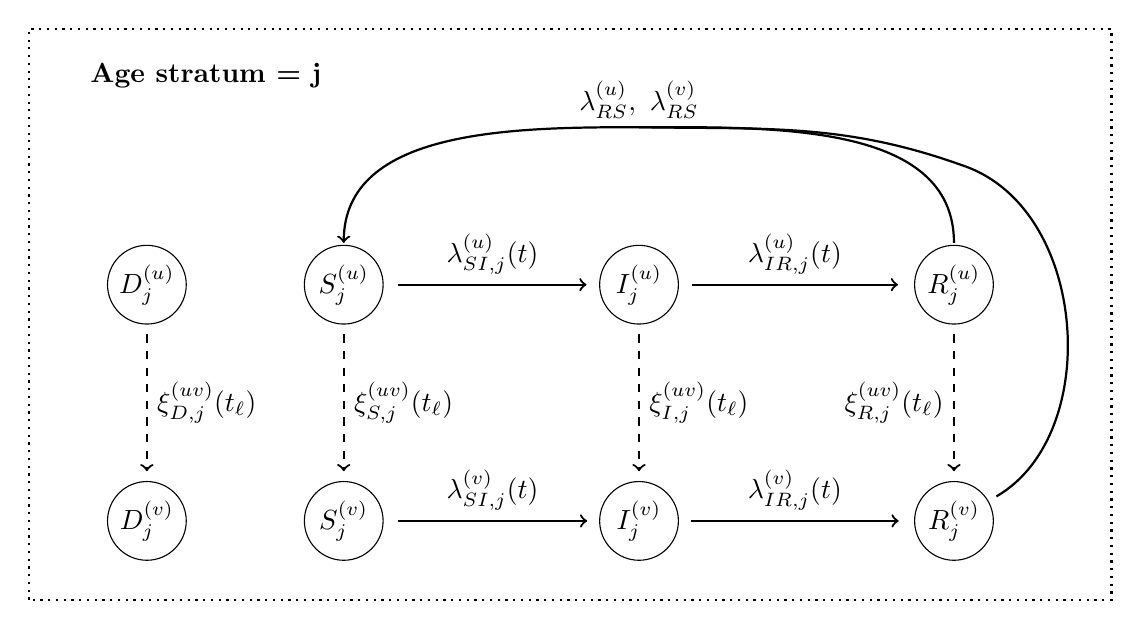
\begin{tikzpicture}
	\draw[thick,dotted] (-2.75,1) rectangle (11,8.25);
	\node at (-0.5,7.25) [label={\textbf{Age stratum = j}}] {};
	\draw (-1.25,5) circle(0.5) node (Dju) {$D_j^{(u)}$};
	\draw (1.25,5) circle(0.5) node (Sju) {$S_j^{(u)}$};
	\draw (5,5) circle(0.5) node (Iju) {$I_j^{(u)}$};
	\draw (9,5) circle(0.5) node (Rju) {$R_j^{(u)}$};
	\draw (-1.25,2) circle(0.5) node (Djv) {$D_j^{(v)}$};
	\draw (1.25,2) circle(0.5) node (Sjv) {$S_j^{(v)}$};
	\draw (5,2) circle(0.5) node (Ijv) {$I_j^{(v)}$};
	\draw (9,2) circle(0.5) node (Rjv) {$R_j^{(v)}$};
	\draw (5,7) coordinate (rec) {};
	\draw (5,7.35) node (reclab) {$ \lambda_{RS}^{(u)},\ \lambda_{RS}^{(v)} $};
	\draw (9.15,6.5) coordinate (rec2) {};
	
	\draw [thick,shorten >=0.25cm,shorten <=0.25cm,->] (Sju) -- (Iju) node[midway,above] {$ \lambda_{SI,j}^{(u)}(t) $};
	\draw [thick,shorten >=0.25cm,shorten <=0.25cm,->] (Iju) -- (Rju) node[midway,above] {$ \lambda_{IR,j}^{(u)}(t) $};
	\draw [thick,shorten >=0.25cm,shorten <=0.25cm,->] (Sjv) -- (Ijv) node[midway,above] {$ \lambda_{SI,j}^{(v)}(t) $};
	\draw [thick,shorten >=0.25cm,shorten <=0.25cm,->] (Ijv) -- (Rjv) node[midway,above] {$ \lambda_{IR,j}^{(v)}(t) $};
	
	\draw [dashed,thick,shorten >=0.25cm,shorten <=0.25cm,->] (Dju) -- (Djv) node[midway,right] {$ \xi_{D,j}^{(uv)}(t_\ell) $};
	\draw [dashed,thick,shorten >=0.25cm,shorten <=0.25cm,->] (Sju) -- (Sjv) node[midway,right] {$ \xi_{S,j}^{(uv)}(t_\ell) $};
	\draw [dashed,thick,shorten >=0.25cm,shorten <=0.25cm,->] (Iju) -- (Ijv) node[midway,right] {$ \xi_{I,j}^{(uv)}(t_\ell) $};
	\draw [dashed,thick,shorten >=0.25cm,shorten <=0.25cm,->] (Rju) -- (Rjv) node[midway,left] {$ \xi_{R,j}^{(uv)}(t_\ell) $};
	
	\draw [thick,shorten >=0cm,shorten <=0.15cm] (Rju) to [out=90, in = 0] (rec);
	\draw [thick,shorten >=0cm,shorten <=0.1cm] (Rjv) to [out=30, in = -20] (rec2);
	\draw [thick] (rec2) to [out=160,in=-1] (rec);
	\draw [thick,shorten >=0.15cm,shorten <=0.0cm,->] (rec) to [out=180, in = 90] (Sju);
	\end{tikzpicture}
	\caption[Diagram of state transitions for an age--vaccination stratified SIRS model for influenza.]{Diagram of state transitions for an age--vaccination stratified SIRS model for influenza in Finland. Both age strata, 0--19 and 20+, have the same compartmental structure. Nodes in circles denote model compartments, which are subscripted with age stratum and superscripted with vaccination status. Solid lines indicate stochastic transitions that occur continuously in time. Rates of disease state transitions, denoted by $ \lambda $, are subscripted with the states from which, and to which, individuals flow and by the age stratum. Superscripts for transition rates indicate vaccination status. Dashed lines represent deterministic forcings from unvaccinated to vaccinated compartments that occur at discrete times. The mass of the forcing at time $ t $, denoted $ \xi(t) $, is subscripted by the compartment and age stratum, and superscripted by the direction of the forcing (unvaccinated to vaccinated).} 
	\label{fig:flu_sirs_diag}
\end{figure}

The contact rate between individuals in age stratum $ j $ and age stratum $ k $, denoted $ C_{jk} $, was based on estimated mean contact rates, appropriately standardized (see Section \ref{sec:flu_contact_rates}), from the Finnish arm of the POLYMOD survey \cite{mossong2008social,polymod} and accessed via the \texttt{socialmixr R} package \cite{funk2018socialmixr}. Sixty percent of contacts in the 0--19 age group were from other individuals age 0--19, while eighty--five percent of the contacts in the 20+ age group were from other adults. The rates, $ \blambda = (\blambda_{Y},\blambda_{A}) $, at which individuals in age--stratum $ j \in \lbrace Y,\ A\rbrace $ transition between disease states are

\begin{equation}\small
\label{eqn:flu_sirs_rates}
\blambda_{j} = \left\lbrace
\begin{array}{ll}
\lambda_{SI,j}^{(u)} = \left [\alpha_{j}(t) + \beta_{j}(t)\left (C_{jk}\left (I_{j}^{(u)} + I_{j}^{(v)}\right ) + (1-C_{jk})\left (I_{k}^{(u)} + I_{k}^{(v)}\right )\right )\right ]S_{j}^{u} \\ 
\lambda_{SI,j}^{(v)} = \nu\left [\alpha_{j}(t) + \beta_{j}(t)\left (C_{jk}\left (I_{j}^{(u)} + I_{j}^{(v)}\right ) + (1-C_{jk})\left (I_{k}^{(u)} + I_{k}^{(v)}\right )\right )\right ]S_{j}^{v}\\
\lambda_{IR,j}^{(u)} = \mu_{j} I_{j}^{(u)} \\
\lambda_{IR,j}^{(v)} = \mu_{j} I_{j}^{(v)} \\
\lambda_{RS,j}^{(u)} = \omega R_{j}^{(u)} \\
\lambda_{RS,j}^{(v)} = \omega R_{j}^{(v)}
\end{array}
\right .
\end{equation}

At weekly intervals, we deterministically force individuals from unvaccinated model compartments to the corresponding vaccinated compartments. Following \cite{shubin2016revealing}, we assume that vaccine doses were distributed proportionally to the number of individuals in each unvaccinated compartment of the corresponding age stratum. In \cite{shubin2016revealing}, it was assumed that vaccination was fully protective with 80\% probability two weeks after administration. Here, we will assume that the vaccine is partially protective in that it reduces the rate at which vaccinated individuals become infected. We do not assume that VE for susceptibility varies by age, and also do not model vaccine efficacy for infectiousness or recovery due to the limited extent of the data. To account for the time required to elicit an immune response, we apply the deterministic forcing at the beginning of week after the time when each dose count was indexed. Suppose that at the end of week $ \ell $ we have $ \bX_j^{(u)}(t_\ell) = \left (S_j^{(u)}(t_\ell),\ I_j^{(u)}(t_\ell),\ R_j^{(u)}(t_\ell),\ D_j^{(u)}(t_\ell)\right ) $ unvaccinated susceptible, infected, recovered, and detached individuals in age stratum $ j $ and $ \bX_j^{(v)}(t_\ell) = \left (S_j^{(v)}(t_\ell),\ I_j^{(v)}(t_\ell),\ R_j^{(v)}(t_\ell),\ D_j^{(v)}(t_\ell\right ) $ vaccinated individuals, and that $ V_j(t_\ell) $ vaccine doses were recorded for stratum $ j $ in that week. We apply the vaccine forcing to the initial state for the following week: 
\begin{align}
\label{eqn:vacc_forcing}
\begin{split}
	\bX_{j}^{(u)}(t_\ell^+) &= \bX_j^{(u)}(t_\ell) - V_j(t_\ell)\frac{\bX_{j}^{(u)}(t_\ell)}{\sum\bX_{j}^{(u)}(t_\ell)}, \\
	\bX_{j}^{(v)}(t_\ell^+) &= \bX_j^{(v)}(t_\ell) + V_j(t_\ell)\frac{\bX_{j}^{(u)}(t_\ell)}{\sum\bX_{j}^{(u)}(t_\ell)}.
\end{split}
\end{align}
Thus, the vaccination forcing affects the initial condition for the period $ (t_\ell,t_{\ell+1}] $, not the state at time $ t_\ell $. 

The diffusion approximation for the MJP is a real--valued process, $ \bX $, that in its infinite population limit evolves as a deterministic system of ODEs. The state space of $ \bX $ is defined in terms of compartment volumes, $ \mcS_X^R $, and with corresponding cumulative incidence process, $ \bN $, with state space $ \mcS_N^R $. Note that the boundary conditions on the state spaces of $ \bX^c $ and $ \bN^c $, and similarly of $ \bX $ and $ \bN $, ensure positivity of compartment counts and monotonicity of cumulative incidence paths, and that the compartment counts each age--vaccination stratum sum to the number of individuals in that stratum, e.g., $ S_{Y}^{(u)}(t) + I_{Y}^{(u)}(t) + R_{Y}^{(u)}(t)+ D_{Y}^{(u)}(t) = N_{Y}^{(u)}(t) $. Due to the complexity of the model, we will rely on the deterministic ODE framework that was explored as a comparitor for the LNA in Chapter \ref{chap:lna_for_sems} to facilitate the computation \ref{chap:lna_for_sems}.  

%As in Chapter \ref{chap:lna_for_sems}, we will use the non--centered parameterization of the restarting LNA of the log--transformed SDE to approximate the time--evolution of $ \bX^c $ and $ \bN^c $. Algorithm \ref{alg:doLNA2} details the procedure for mapping standard normal LNA draws onto an LNA sample path with vaccination forcings.

\subsubsection{Reproduction numbers}
\label{subsubsec:stratmod_repnumbs}
The basic reproduction number, $ R_0 $, and its variants describe the propensity of an outbreak to spread through a population \cite{heffernan2005perspectives,van2008further}. $ R_0 $ is loosely interpreted as the average number of secondary infections arising from a single infected individual in a completely susceptible population. An outbreak will fail to sustain itself (almost surely when it evolves deterministically, but in reality with high probability due to the inherently stochastic nature of epidemics) when $ R_0 < 1 $. For this reason, epidemiologists often quantify the effectiveness of a control measure by estimating the extent to which the intervention reduces $ R_0 $. We can interpret the basic reproduction number as an intrinsic reproduction number when there is an exogenous contribution to force of infection \cite{blackwood2018introduction}. From a modeling perspective, is important to understand not only how $ R_0 $ affects the transmission dynamics, but also how various aspects of the model interact to affect $ R_0 $. 

The basic reproduction number of a structured SEM can be obtained by computing the spectral radius (absolute value of the dominant eigenvalue) of the next generation matrix (NGM) for the linearized system of ODEs specifying the flow in and out of states at infection \cite{heffernan2005perspectives,van2017reproduction,van2008further}. The $ i,j $ element of the NGM gives the expected number of secondary infections in age stratum $ i $ given an index infection in stratum $ j $. Noting that vaccinated and unvaccinated invididuals in this model are equally transmissive and have the same mean infectious period durations, we obtain the age--structured next generation matrix
\begin{align}
\label{eqn:sirs_ngm_full}
\bK &= 
	\left (
	\begin{array}{cc}
	K_{YY} & K_{YA} \\
	K_{AY} & K_{AA}
	\end{array}
	\right ) =\left (
	\begin{array}{cc}
	\frac{C_{YY}\beta_Y\left (N_Y^{(u)} + \nu_YN_Y^{(v)}\right )}{\mu_Y} & \frac{C_{YA}\beta_Y\left (N_Y^{(u)} + \nu_YN_Y^{(v)}\right )}{\mu_A} \\[2ex]
	\frac{C_{AY}\beta_A\left (N_A^{(u)} + \nu_AN_A^{(v)}\right )}{\mu_Y} & \frac{C_{AA}\beta_A\left (N_A^{(u)} + \nu_AN_A^{(v)}\right )}{\mu_A}
	\end{array}
	\right ).
\end{align}
The basic reproduction number is 
\begin{align}
\label{eqn:sirs_R0}
R_0 = \frac{1}{2}\left (K_{YY} + K_{AA}\right ) + \frac{1}{2}\sqrt{(K_{YY} - K_{AA})^2 + 4K_{YA}K_{AY}}.
\end{align}

Note that is possible for the outbreak to persist, i.e., $ R_0 > 1 $,  when the intrinsic reproduction number in one of the strata is below 1, e.g., $ K_{YY} <1$, even though most transmission arises from within--group contacts. However, $ R_0 <$ will be less than 1 if both $ K_{YY} <1 $ and $ K_{AA} <1 $.

Furthermore, the basic reproduction number is greater than the average of intrinsic reproduction numbers, $ K_{YY} $ and $ K_{AA} $, since the second term on the right hand side of (\ref{eqn:sirs_R0}) will typically be positive. Similarly, the variance of $ R_0 $ is also greater than the average of variances of $ K_{YY} $ and $ K_{AA} $. For these reasons, we should consider how $ K_{YY} $ and $ K_{AA} $ interact to induce a prior over $ R_0 $ when parameterizing the model. Note that if the cross--stratum contact rates were negligible, $ R_0 $ would behave like the average of intrinsic reproduction numbers plus a term proportional to the absolute difference between $ K_{YY} $ and $ K_{AA} $. This suggests that prior information about the intrinsic reproduction numbers, either individually (our preference) or about their average and difference, could help identify $ R_0 $. We should also keep in mind that our model is more complicated since the cross stratum terms are not negligible ($ C_{AA} = 0.6 $, $ C_{YY}=0.85 $), hence
\begin{align*}
K_{YA} &= \frac{(1 - C_{YY})}{C_{YY}}\frac{\mu_Y}{\mu_A}K_{YY},\hspace{0.25in}
K_{AY} = \frac{(1 - C_{AA})}{C_{AA}}\frac{\mu_A}{\mu_Y}K_{AA},\\
&\implies K_{YA}K_{AY} = \frac{(1 - C_{YY})(1-C_{AA})}{C_{YY}C_{AA}}K_{YY}K_{AA}.
\end{align*} 
Thus, $ R_0 $ is the average of $ K_{YY} $ and $ K_{AA} $, plus a non--linear function of $ K_{YY} $ and $ K_{AA} $.

Finally we emphasize the importance of accounting for all of the parameters that contribute the intrinsic reproduction numbers, and by extension $ R_0 $, when specifying priors and parameterizing the estimation scale of the MCMC. In particular, it is critical to note that the effective population size might be lower than the nominal population size because of vaccination and depletion of susceptibles. We can easily misspecify the scales of prior distributions for the reproduction numbers, or select an inefficient parameterization for the MCMC estimation scale, by neglecting this dynamic. In our model, for example, the value of $ R_0 $ in the first season, and the rate at which recovered individuals lose immunity, will affect the effective population size at the beginning of the second season. 

\subsection{Flexible Models for the Force of Infection with Gaussian Markov Random Fields}
\label{subsec:flu_gmrf}

We will model the time--varying force of infection using first order GMRFs for the log intrinsic reproduction numbers and the effective rate of exogenous infectious contacts in each age stratum. The GMRFs are separately specified over three epochs corresponding to the period one month before the first detected case until the start of the Finnish school year in 2009, the beginning of the Finnish school year in 2009 until its start in 2010 (including the inter--season period), and the second epidemic season beginning at the start of the Finnish school year, 2010. These epochs correspond to epiweeks 15, 2009 through epiweek 34, 2009, epiweek 35, 2009 through epiweek 32, 2010, and epiweek 33, 2010 through epiweek 22, 2011. We will assume that the intrinsic reproduction numbers are homogeneous over the inter--season period, from epiweek 16, 2010 -- epiweek 32, 2010.

Let $ \bpsi_{j} = \lbrace\psi_{j,\ell}:\ \ell \in 0,\dots,52,71,\dots,112\rbrace $ be the vector of intrinsic reproduction numbers for stratum $ j \in \lbrace Y,A \rbrace$, ignoring the relative contact rates, $ C_{jk} $, and vaccination. The reproduction number in time interval $ \ell $, indexed in weeks from epiweek 15, 2009, is
\begin{equation}
\label{eqn:R0t_novacc}
\psi_{j,\ell} = \frac{\beta_j(t_\ell)N_js_j}{\mu_j},
\end{equation}
where $ \beta_j(t_\ell) $ is the per--contact infection rate, $ \mu_j $ is the recovery rate, $ N_j $ is the size of the age stratum, and $ s_j $ is the fraction of individuals in stratum $ j $ that are susceptible.
 
When transmission is sustained at near--endemic levels, we should expect that the effective reproduction numbers are near one, or perhaps slightly above. Let $ \nu $ be the relative rate of infectious contact among vaccinated individuals, i.e., one minus the vaccine efficacy for susceptibility. The effective reproduction number, which accounts for the effects of vaccination and depletion of susceptibles, is 
\begin{equation}
\label{eqn:Reff_t}
\psi_{j,\ell}^{eff} = \frac{\beta_j(t_\ell)_j\left (S^{(u)}_j(t_\ell) + S^{(v)}_j(t_\ell)\nu\right )}{\mu_j}
\end{equation}
If vaccination does not increase the rate of infectious contact (and we will assume it does not), then $ \psi_{j,\ell}^{eff} < \psi_{j,\ell} $ since $ \nu\in[0,1] $ and $ (S^{(u)}_j(t_\ell) + S^{(v)}_j(t_\ell) < N_js_j $. It is critical to account for this when specifying priors for the basic intrinsic reproduction numbers at the start of each epoch. It would not do, for instance, to set priors for the intrinsic basic reproduction numbers at the beginning of the third epoch that nominally concentrate mass near one since this would imply that the effective reproduction numbers are far below one due to vaccination and depletion of susceptibles during the first wave of the outbreak. Our approach will be to assign priors to the vaccination adjusted intrinsic reproduction numbers at the beginning of each epoch, $ \psi_{j,\ell}^\prime = \psi_{j,\ell}  \left (1 - P^v_j(t_\ell) + P^v_j(t_\ell)\right ) $, where $ P_j^v(t_\ell) $ is the vaccination coverage in stratum $ j $ at $ t_\ell $. 

We denote by $ \Delta $ the first--order forward difference operator, i.e., $ \Delta X_j = X_{j+1} - X_j $. The first--order differences of the log intrinsic reproduction numbers for stratum $ j $ in each epoch are assigned a Gaussian prior with mean zero and variance $ \sigma^2_{j,\ell} $. The sub--model for intrinsic reproduction numbers in stratum $ j $ is

\begin{small}
	\begin{align}
	\log(\psi_{j,\ell}) &\sim \mcN(\mu_{j,\ell},\tau_{j,\ell}^2),&\ &\ell= 0,19,71, \nonumber\\
	\log(\sigma_{j,\ell}) &\sim \mcN(m_{j,\ell}, s_{j,\ell}^2),&\ &\ell=0,19,71, \nonumber\\
	\Delta\log(\psi_{j,\ell})&\sim \mcN(0, \sigma^2_{j,0}),&\ &\ell=0,\dots,17, \nonumber\\
	\Delta\log(\psi_{j,\ell})&\sim \mcN(0, \sigma^2_{j,19}),&\ &\ell=19,\dots,51, \nonumber\\
	\Delta\log(\psi_{j,\ell})&\sim \mcN(0, \sigma^2_{j,71}),&\ &\ell=71,\dots,111, \nonumber\\
	\log(\psi_{j,\ell}) &= \log(\psi_{j,0}) + \sum_{k=0}^{\ell-1}\Delta\log(\psi_{j,k}),&\ &\ell = 1,\dots,17, \nonumber\\
	\log(\psi_{j,\ell}) &= \log(\psi_{j,19}) + \sum_{k=0}^{\ell-1}\Delta\log(\psi_{j,19+k}),&\ &\ell = 19,\dots,52, \nonumber\\
	\log(\psi_{j,\ell}) &= \log(\psi_{j,71}) + \sum_{k=0}^{\ell-1}\Delta\log(\psi_{j,71+k}),&\ &\ell = 72,\dots,112. \nonumber \\
	\beta_j(t_\ell) &= \psi_{j,\ell}N_j/\left (\mu_{j}(t_\ell)(1 - P^v_j(t_\ell) + P_j^v(t_\ell)\nu_j)\right ),&\ &\ell=0,\dots,52,71,\dots,112. \nonumber
	\end{align}
\end{small}

The induced GMRF prior for the vaccination adjusted basic reproduction numbers is given in Figure \ref{fig:flurw1prior}. 

In practice, we will use the following partially non--centered parameterization:
\begin{small}
	\begin{align}
	\log(\psi_{j,\ell}) &\sim \mcN(\mu_{j,\ell},\tau_{j,\ell}^2),&\ &\ell= 0,19,71, \nonumber\\
	Z_{\log(\sigma_{j,\ell})} &\sim \mcN(0,1),&\ &\ell=0,19,71, \nonumber \\
	Z_{\Delta\log(\psi_{j,\ell})} &\sim \mcN(0,1),&\ &\ell=0,\dots,17,19,\dots,51,71,\dots,111, \nonumber \\ 
	\log(\sigma_{j,\ell}) &= m_{j,\ell} + s_{j,\ell}Z_{\log(\sigma_{j,\ell})},&\ &\ell = 0,19,71,\nonumber\\
	\Delta\log(\psi_{j,\ell})&= \sigma_{j,0} Z_{\Delta\log(\psi_{j,\ell})},&\ &\ell=0,\dots,17, \nonumber\\
	\Delta\log(\psi_{j,\ell})&= \sigma_{j,19} Z_{\Delta\log(\psi_{j,\ell})},&\ &\ell=19,\dots,51, \nonumber\\
	\Delta\log(\psi_{j,\ell})&= \sigma_{j,71} Z_{\Delta\log(\psi_{j,\ell})},&\ &\ell=71,\dots,111, \nonumber\\
	\log(\psi_{j,\ell}) &= \log(\psi_{j,0}) + \sum_{k=0}^{\ell-1}\Delta\log(\psi_{j,k}),&\ &\ell = 1,\dots,17, \nonumber\\
	\log(\psi_{j,\ell}) &= \log(\psi_{j,19}) + \sum_{k=0}^{\ell-1}\Delta\log(\psi_{j,19+k}),&\ &\ell = 19,\dots,52, \nonumber\\
	\log(\psi_{j,\ell}) &= \log(\psi_{j,71}) + \sum_{k=0}^{\ell-1}\Delta\log(\psi_{j,71+k}),&\ &\ell = 72,\dots,112. \nonumber \\
	\beta_j(t_\ell) &= \psi_{j,\ell}N_j/\left (\mu_{j}(t_\ell)(1 - P^v_j(t_\ell) + P_j^v(t_\ell)\nu_j)\right ),&\ &\ell=0,\dots,52,71,\dots,112. \nonumber
	\end{align}
\end{small}

We similarly assign a first order GMRF prior to the effective number of exogenous infectious contacts for each age stratum. Note that this term is somewhat of a catch--all for infectious contacts that arise outside of the density dependent mixing of susceptible and infected individuals. The rate of exogenous infection may be loosely interpreted as either the baseline rate of infectious contact or as the rate of infection from outside the population. Let $ \alpha^\prime_{j,\ell} = \alpha_{j,\ell}N_js_j $ denote the rate of exogenous infection for age stratum $ j $ in week $ \ell $, scaled by the effective stratum size. The GMRF prior for $ \balpha^\prime_j = \lbrace\alpha^\prime_{j,\ell}:\ \ell=0,\dots,52,71,\dots,112\rbrace $ is
\begin{small}
	\begin{align}
	\log(\alpha^\prime_{j,\ell}) &\sim \mcN(\mu_{j,\ell},\tau_{j,\ell}^2),&\ &\ell= 0,19,71, \nonumber\\
	\log(\sigma_{j,\ell}) &\sim \mcN(m_{j,\ell}, s_{j,\ell}^2),&\ &\ell=0,19,71, \nonumber\\
	\Delta\log(\alpha^\prime_{j,\ell})&\sim \mcN(0, \sigma^2_{j,0}),&\ &\ell=0,\dots,17, \nonumber\\
	\Delta\log(\alpha^\prime_{j,\ell})&\sim \mcN(0, \sigma^2_{j,19}),&\ &\ell=19,\dots,51, \nonumber\\
	\Delta\log(\alpha^\prime_{j,\ell})&\sim \mcN(0, \sigma^2_{j,71}),&\ &\ell=71,\dots,111, \nonumber\\
	\log(\alpha^\prime_{j,\ell}) &= \log(\alpha^\prime_{j,0}) + \sum_{k=0}^{\ell-1}\Delta\log(\alpha^\prime_{j,k}),&\ &\ell = 1,\dots,17, \nonumber\\
	\log(\alpha^\prime_{j,\ell}) &= \log(\alpha^\prime_{j,19}) + \sum_{k=0}^{\ell-1}\Delta\log(\alpha^\prime_{j,19+k}),&\ &\ell = 19,\dots,52, \nonumber\\
	\log(\alpha^\prime_{j,\ell}) &= \log(\alpha^\prime_{j,71}) + \sum_{k=0}^{\ell-1}\Delta\log(\alpha^\prime_{j,71+k}),&\ &\ell = 72,\dots,112. \nonumber \\
	\alpha_{j,\ell} &= \alpha^\prime_{j,\ell}/N,&\ &\ell=0,\dots,52,71,\dots,112. \nonumber
	\end{align}
\end{small}

Again, we will use a partially non--centered parameterization in practice.
\begin{small}
	\begin{align}
	\log(\alpha^\prime_{j,\ell}) &\sim \mcN(\mu_{j,\ell},\tau_{j,\ell}^2),&\ &\ell= 0,19,71, \nonumber\\
	Z_{\log(\sigma_{j,\ell})} &\sim \mcN(0,1),&\ &\ell=0,19,71, \nonumber \\
	Z_{\Delta\log(\alpha^\prime_{j,\ell})} &\sim \mcN(0,1),&\ &\ell=0,\dots,17,19,\dots,51,71,\dots,111, \nonumber \\ 
	\log(\sigma_{j,\ell}) &= m_{j,\ell} + s_{j,\ell}Z_{\log(\sigma_{j,\ell})},&\ &\ell = 0,19,71,\nonumber\\
	\Delta\log(\alpha^\prime_{j,\ell})&= \sigma_{j,0} Z_{\Delta\log(\alpha^\prime_{j,\ell})},&\ &\ell=0,\dots,17, \nonumber\\
	\Delta\log(\alpha^\prime_{j,\ell})&= \sigma_{j,19} Z_{\Delta\log(\alpha^\prime_{j,\ell})},&\ &\ell=19,\dots,51, \nonumber\\
	\Delta\log(\alpha^\prime_{j,\ell})&= \sigma_{j,71} Z_{\Delta\log(\alpha^\prime_{j,\ell})},&\ &\ell=71,\dots,111, \nonumber\\
	\log(\alpha^\prime_{j,\ell}) &= \log(\alpha^\prime_{j,0}) + \sum_{k=0}^{\ell-1}\Delta\log(\alpha^\prime_{j,k}),&\ &\ell = 1,\dots,17, \nonumber\\
	\log(\alpha^\prime_{j,\ell}) &= \log(\alpha^\prime_{j,19}) + \sum_{k=0}^{\ell-1}\Delta\log(\alpha^\prime_{j,19+k}),&\ &\ell = 19,\dots,52, \nonumber\\
	\log(\alpha^\prime_{j,\ell}) &= \log(\alpha^\prime_{j,71}) + \sum_{k=0}^{\ell-1}\Delta\log(\alpha^\prime_{j,71+k}),&\ &\ell = 72,\dots,112. \nonumber \\
	\alpha_{j,\ell} &= \alpha^\prime_{j,\ell}/N,&\ &\ell=0,\dots,52,71,\dots,112 \nonumber
	\end{align}
\end{small}

The initial reproduction numbers, for which we retain the centered parameterization, are blocked with other model parameters and updated using a multivariate normal slice sampler (MVNSS). The non--centered GMRF differences and their standard deviations are updated 
%jointly with the LNA path 
using elliptical slice sampling (Algorithm \ref{alg:elliptical_slice_sampler}).
%(Algorithm \ref{alg:elliptss_lna_gmrf}). 
Readers familiar with GMRFs will note the, somewhat unconventional, Gaussian prior for the standard deviation of the GMRF increments. This choice was made for computational reasons in order to facilitate joint updates of the GMRF and its hyper--parameters. Alternating between field and hyper--parameter updates is known to results in poorly mixing MCMC chains as large updates to the hyper--parameters quickly result in fields that are not concordant with the data  \cite{knorr2002block,murray2010hyper}. 

\subsection{Sampling from the Posterior}
\label{subsec:flu_mcmc}

Let $ \bZ = \left (\bZ^F,\bZ^{\btheta_F}\right ) $ denote the vector of i.i.d. standard normal draws for the GMRF increments and GMRF hyperparameters, $ \doGMRF(\bZ;\btheta) $ be the operation for computing the GMRF from its draws and hyperparameters, and $ \pi(\btheta) $ be the prior distributions for the other model parameters. Let $ \mathcal{T} = \lbrace t_\ell:\ \ell = 1,\dots,52,71,\dots,113 \rbrace $ denote the set of observation times. Our MCMC will target the posterior
\begin{align}
\label{eqn:flu_posterior}
\pi(\btheta,\bZ | \bY) &\propto \pi(\bZ)\pi(\btheta)\pi(\bY|\btheta,\bZ) \nonumber\\
&= \pi(\bZ)\pi(\btheta) \prod_{t_\ell\in\mathcal{T}}\prod_{j\in\lbrace Y,A\rbrace} \Pr\left (Y_{j}(t_\ell) | \doGMRF(\bZ),\btheta,\mcI)\right )
\end{align}
MCMC proceeds by alternately updating $ \bZ|\bY,\btheta $ using ElliptSS (Algorithm \ref{alg:elliptss_lna_gmrf}) and MVNSS updates for $ \btheta|\bY,\bZ $ (Algorithm \ref{alg:mvnss}). Priors for model parameters were informative are detailed in Section \ref{subsec:flu_priors} and additional MCMC details are provided in Section \ref{subsec:flu_mcmc_details}. Generally speaking, priors for parameters were informative and we made an effort to choose priors that were based on published estimates from other studies.

%Let $ \bZ = \left (\bZ^X,\bZ^F,\bZ^{\btheta_F}\right ) $ denote the vector of i.i.d. standard normal draws for the LNA, GMRF increments, and GMRF hyperparameters, and let $ \pi(\btheta) $ be the prior distributions for the other model parameters. Let $ \mathcal{T} = \lbrace t_\ell:\ \ell = 1,\dots,52,71,\dots,113 \rbrace $ denote the set of observation times. Our MCMC will target the posterior
%\begin{align}
%\label{eqn:flu_posterior}
%\pi(\btheta,\bZ | \bY) &\propto \pi(\bZ)\pi(\btheta)\pi(\bY|\btheta,\bZ) \nonumber\\
%&= \pi(\bZ)\pi(\btheta) \prod_{t_\ell\in\mathcal{T}}\prod_{j\in\lbrace Y,A\rbrace} \Pr\left (Y_{j}(t_\ell) | \doLNA2(\bZ,\btheta,\mcI,\bxi)\right )
%\end{align}
%MCMC proceeds by alternately updating $ \bZ|\bY,\btheta $ using ElliptSS (Algorithm \ref{alg:elliptss_lna_gmrf}) and MVNSS updates for $ \btheta|\bY,\bZ $ (Algorithm \ref{alg:mvnss}). 

\section{Results}
\label{sec:flu_results}

\subsection{Incidence}
\label{subsec:flu_incid_res}
Estimates of cumulative incidence and attack rates by season and age group are reported in Table \ref{tab:flu_attack_rates}. We estimate that there were approximately 532,000 (95\% BCI: 393,000, 703,000) infections in the first epidemic season, and an additional 240,000 (95\% BCI: 172,000, 333,000) cases during the second season. These estimates would correspond to estimated attack rates of 7.4\%--13.1\% during the first season, and 3.2\%--6.2\% in the second season if each individual was infected only once. The estimated attack rates were substantially higher among youths than adults in the first epidemic season, and slightly higher during the second season. The estimated incidence over the inter--season period was low; 110 cases (95\% BCI: 50, 250) among youths, and 330 cases (95\% BCI: 150, 710) among adults. 

\begin{sidewaystable}[htbp]
	\caption{Estimated infections (thousands) and attack rates by season and age stratum. Attack rates are calculated as the number of infections divided by the size of each stratum, assuming that cases are unique.}
	\label{tab:flu_attack_rates}
	\centering\footnotesize
	\begin{tabular}{lrrrrrr}
		\hline
		&\multicolumn{6}{c}{\textbf{Time varying dynamics}}\\
		\cmidrule{2-7} & \multicolumn{2}{c}{\textit{Season 1}} & \multicolumn{2}{c}{\textit{Season 2}} & \multicolumn{2}{c}{\textit{Both Seasons}}\\
		\cmidrule(r){2-3}\cmidrule(lr){4-5}\cmidrule(l){6-7} & 
		Incidence & Attack rate & Incidence & Attack rate & Incidence & Attack rate \\
		\hline
	Ages 0-19 & 174 (127, 231) & 14.2 (10.4, 18.9) & 68.6 (46.6, 100) & 5.6 (3.8, 8.2) & 244 (181, 321) & 19.9 (14.8, 26.2)\\
	Ages 20+ & 356 (243, 501) & 8.6 (5.9, 12.1) & 171 (117, 245) & 4.1 (2.8, 5.9) & 530 (378, 720) & 12.8 (9.2, 17.4)\\
	All ages & 532 (393, 703) & 9.9 (7.4, 13.1) & 240 (172, 333) & 4.5 (3.2, 6.2) & 774 (586, 1,010) & 14.5 (11, 18.8)\\
		\hline &&&&&&\\
		&\multicolumn{6}{c}{\textbf{Piecewise homogeneous dynamics}}\\
		\cmidrule{2-7}	& \multicolumn{2}{c}{\textit{Season 1}} & \multicolumn{2}{c}{\textit{Season 2}} & \multicolumn{2}{c}{\textit{Both Seasons}}\\
	\cmidrule(r){2-3}\cmidrule(lr){4-5}\cmidrule(l){6-7} & 
	Incidence & Attack rate & Incidence & Attack rate & Incidence & Attack rate \\
	\hline
	Ages\_0-19 & 150 (107, 203) & 12.3 (8.7, 16.6) & 55.1 (34.4, 82) & 4.5 (2.8, 6.7) & 206 (154, 267) & 16.8 (12.6, 21.9)\\
	\hline
	Ages\_20+ & 263 (182, 375) & 6.4 (4.4, 9.1) & 181 (128, 242) & 4.4 (3.1, 5.9) & 445 (324, 598) & 10.8 (7.9, 14.5)\\
	\hline
	All\_ages & 414 (305, 556) & 7.7 (5.7, 10.4) & 236 (178, 309) & 4.4 (3.3, 5.8) & 653 (499, 840) & 12.2 (9.3, 15.7)\\
		\hline
	\end{tabular}
\end{sidewaystable}

\subsection{Transmission Dynamics}
\label{flu_res_dynamics}
Estimates of time varying reproduction numbers and exogenous infections are shown in Figure \ref{fig:flurwodetimevaryingplots} and estimates of model parameters are given in Table \ref{tab:flu_param_ests}. The period just prior to the first detected cases until the start of the Finnish school year in 2009 was characterized by low basic and effective reproduction numbers. The basic reproduction numbers over this period remained at near--endemic levels (95\% BCI: 0.99, 1.00; second and third rows of Figure \ref{fig:flurwodetimevaryingplots}). 

The basic reproduction numbers from the start of the Finnish school year through the peak of the first wave of the outbreak were somewhat higher at around 1.2 (95\% BCI: 1.1, 1.3), increased slightly as the epidemic peaked, but declined below one in early December, 2009, as a result in vaccination. Incidence began to decline, starting in mid--November, preceding the drop in basic reproduction numbers due to vaccination by several weeks, and well before vaccine coverage had reached meaningful levels. The effective reproduction numbers declined throughout the first wave, indicating that the slight increases in rates of infectious contact overwhelmed by depletion of susceptibles.

The vaccination--adjusted basic reproduction numbers at the start of the second season, roughly 1.4 (95\% BCI: 1.3, 1.6), were nominally higher than at the start of the first season. However, these estimates do not account for depletion of susceptibles in the first wave of the outbreak. Effective reproduction numbers at the beginning of second epidemic wave were roughly 1.16 (95\% BCI: 1.10, 1.23), were comparable to effective reproduction numbers during the first wave. Without adjusting for vaccination, the basic reproduction numbers would be in the range of 2.4--4, which is similar to results in \cite{shubin2016revealing}. Accounting for vaccination and depletion of susceptibles brings the adjusted reproduction numbers into the range that is more similar to previous estimates for A(H1N1)pdm09 outbreaks \cite{biggerstaff2014estimates}. 

Figure \ref{fig:flurwodetimevaryingplots} presents the effective and vaccine adjusted type reproduction numbers for the 0--19 and 20+ age strata, which are interpreted as the expected number of secondary cases of any age caused by a single index case in a given age stratum. The type reproduction numbers are the column sums of the basic (vaccine adjusted) and effective NGMs. Note that this definition differs from the definition of type reproduction number in \cite{heesterbeek2007type}, which is the expected number of secondary cases of a particular type given an index case of that type. At the beginning of the first epidemic wave (epiweek 34, 2009), an index youth case was estimated to result in 1.3 (95\% BCI: 1.0, 1.6) secondary cases, while an index adult would result in 1.15 (95\% BCI: 1.0, 1.3) secondary cases. The contribution of youths to the FOI declined dramatically in the second season, while the contribution of adults was roughly the same. At the start of the second season, an index youth case was estimated to lead to 1.0 (95\% BCI: 0.8, 1.25) secondary cases, while an index adult case to 1.2 (1.0, 1.3) secondary cases. The change in the role contribution of youths in the second season can be attributed to the depletion of susceptible youths in the first season due to vaccination and high attack rates in that season. The effective type reproduction numbers in both age strata decline throughout the first wave, while in the second season they increase slightly before again declining as susceptibles deplete. The slight uptick in effective type reproduction numbers at the end of the second season is attributable to loss of immunity among previously infected individuals.  

\begin{sidewaysfigure}[htbp]
	\centering
	\includegraphics[width=0.95\linewidth]{figures/flu_rw_ode_timevarying_plots}
	\caption{Posterior estimates of time varying quantities under time varying dynamics. Estimated incidence (top row), effective reproduction numbers (second row), vaccination adjusted basic reproduction numbers (third row), and exogenous infections (bottom row). $ N_{SI}^j(t), $ is the weekly incidence in age stratum $ j $, $ R_{eff}(t) $ and $ R_{adj}(t) $ are the effective and vaccination--adjusted basic reproduction numbers, $ T_{eff}^j(t) $ is the type reproduction number for stratum $ j $ (expected \# of secondary infections in all strata for a single infected in stratum $ j $), and $ \alpha_j(t) $ is the rate of exogenous infectious contacts for stratum $ j $.}
	\label{fig:flurwodetimevaryingplots}
\end{sidewaysfigure}

The mean infectious period of youths was substantially longer that of adults, 6.5 days (95\% BCI: 4.3 days, 8.8 days) compared with 2.6 days (1.9 days, 3.4 days), respectively. Published point estimates of the serial interval for A(H1N1)pdm09, which is the average time between an index case and a secondary case, and which we might expect to be a bit shorter than the mean infectious period, have mostly been in the 2--3.5 day range \cite{vink2014serial}. Immunity following infection was relatively long--lasting, although a sizable percentage of individuals who were infected lost immunity; 8.2\% (95\% BCI: 3.8\%, 16.2\%) of individuals who had become infected before the start of the second season had lost protection by the beginning of the second season, while the percentage of infected individuals who became infected over both seasons and lost immunity by the end of season two was 10.6\% (95\% BCI: 5.0\%, 19.9\%). The vaccine was estimated to be quite effective,  reducing the rate of infectious contact by 95\% (95\% BCI: 83\%, 99\%). 

\begin{sidewaystable}[htbp]
	\caption[Posterior estimates of SIRS model parameters for pandemic A(H1N1) influenza in Finland.]{Posterior estimates of SIRS model parameters for pandemic A(H1N1) influenza in Finland. Intrinsic reproduction numbers account for vaccine coverage and vaccine efficacy via (\ref{eqn:R0t_vacc}).} 
	\label{tab:flu_param_ests}
	\centering\footnotesize
	\begin{tabular}{clrr}
		\hline
		&&\multicolumn{2}{c}{\textbf{Dynamics}}\\
		\cmidrule{3-4}\textbf{Parameter} & \textbf{Interpretation} & \textit{Time varying} & \textit{Piecewise homogeneous}\\
		\hline
		$ \psi_{Y,0} $ & Intrinsic $ R_0 $ for youths at epiweek 15, 2009  & 1.1 (1.0, 1.2) & 1.1 (1.0, 1.2)\\
		$ \psi_{Y,18} $ & Intrinsic $ R_0 $ for youths at epiweek 34, 2009 & 1.5 (1.1, 1.8) & 1.6 (1.3, 1.9)\\
		$ \psi_{Y,71} $ & Intrinsic $ R_0 $ for youths at epiweek 33, 2010 & 1.2 (0.93, 1.5) & 1.2 (0.94, 1.5)\\
		$ \psi_{A,0} $ & Intrinsic $ R_0 $ for adults at epiweek 15, 2009  & 1.1 (1, 1.2) & 1.1 (1, 1.1)\\
		$ \psi_{A,18} $ & Intrinsic $ R_0 $ for adults at epiweek 34, 2009 & 1.1 (0.95, 1.2) & 1.1 (0.96, 1.2)\\
		$ \psi_{A,71} $ & Intrinsic $ R_0 $ for adults at epiweek 33, 2010 & 1.4 (1.1, 1.8) & 1.6 (1.4, 1.8)\\
		$ 1/\mu_{Y} $ & Mean infectious period for youths (days) & 6.5 (4.3, 8.8) & 7.5 (5.5, 9.5)\\
		$ 1/\mu_A $ & Mean infectious period for adults (days) & 2.6 (1.9, 3.4) & 2.9 (2.2, 3.8)\\
		$ 1/\mu $ & Mean duration of immunity (years) & 9.3 (4.5, 21) & 9.9 (4.8, 21)\\
		$ \nu $ & 1 - VE for susceptibility & 0.05 (0.01, 0.17) & 0.04 (0.01, 0.13)\\
		$ \rho_Y $ & Mean case detection rate for youths & 0.008 (0.006, 0.012) & 0.008 (0.006, 0.011)\\
		$ \rho_A $ & Mean case detection rate for adults & 0.003 (0.002, 0.005) & 0.003 (0.002, 0.004)\\		
		$ 1/\sqrt{\phi_Y} $ & Negative binomial overdispersion for youths & 0.99 (0.82, 1.2) & 1 (0.85, 1.3)\\
		$ 1/\sqrt{\phi_A} $ & Negative binomial overdispersion for adults & 0.97 (0.83, 1.2) & 1 (0.83, 1.2)\\
		\hline
	\end{tabular}
\end{sidewaystable}

The posterior predictive distributions for cases (Figure \ref{fig:flupostpredsrwode}) suggests that the model does a better job reconstructing the second epidemic season than the first, particularly among individuals ages 0--19. The model seems to substantially underestimate the peak of the outbreak in the first season. This might seem somewhat surprising given that the attack rates in the first season were quite high. One possibility is that heterogeneity in detection rates is confounding our estimates of the unobserved epidemic process. In their analysis of this data, \cite{shubin2016revealing} estimated that detection was positively associated with incidence. It is also possible that misspecification of the effective population size could be contributing to the lack of model fit. This might occur, for example, if a meaningful percentage of the population were geographically separated from the areas with intense transmission, or were immune due to exposure to A(H1N1) early in life (as might be the case for older individuals who had antibodies from the 1918 pandemic).  

\begin{figure}[htbp]
	\centering
	\includegraphics[width=\linewidth]{figures/flu_postpreds_rw_ode}
	\caption{Posterior predictive distributions of a stratified SIRS ODE model with time varying dynamics for A(H1N1)pdm09 in Finland.}
	\label{fig:flupostpredsrwode}
\end{figure}


\subsection{Piecewise Homogeneous Dynamics}
\label{subsec:flu_res_homog}

For comparison, we fit a model where the outbreak dynamics were piecewise homogeneous (PH) in each epoch. The vaccination adjusted basic reproduction number was estimated for each of the three epochs, and the per--contact infection rate computed from the vaccination adjusted basic reproduction number. The rate of exogenous infection was also constant within each epoch, but no other aspects of the model dynamics differed from the previous model. Posterior distributions of time varying quantities are presented in Figure \ref{fig:fluconstodetimevaryingplots}, and posterior estimates of model parameters are summarized in Table \ref{tab:flu_param_ests}. 

\begin{sidewaysfigure}[htbp]
	\centering
	\includegraphics[width=0.95\linewidth]{figures/flu_const_ode_timevarying_plots}
	\caption{Posterior estimates of time varying quantities under piecewise homogeneous dynamics. Estimated incidence (top row), effective reproduction numbers (second row), vaccination adjusted basic reproduction numbers (third row), and exogenous infections (bottom row). $ N_{SI}^j(t), $ is the weekly incidence in age stratum $ j $, $ R_{eff}(t) $ and $ R_{adj}(t) $ are the effective and vaccination--adjusted basic reproduction numbers, $ T_{eff}^j(t) $ is the type reproduction number for stratum $ j $ (expected \# of secondary infections in all strata for a single infected in stratum $ j $), and $ \alpha_j(t) $ is the rate of exogenous infectious contacts for stratum $ j $.}
	\label{fig:fluconstodetimevaryingplots}
\end{sidewaysfigure}


The GMRF and PH models are qualitatively quite similar. Estimated attack rates were comparable, though perhaps slightly higher under the PH model. Estimates of the parameters that govern the model dynamics were also largely in agreement, with dwell times in the infectious and recovered states being slightly longer under the PH model. The rate of exogeneous infections among adults was higher under the PH model in the first epoch, but otherwise comparable. The posterior predictive performance of the PH model is nearly identical to that of the GMRF model (Figure \ref{fig:flu_rw_const_ppicomp}), though PPIs under the PH model tended to be slightly wider. 

On the whole, the similarity between the PH and GMRF models is unsurprising given that the variability of the GMRF was fairly constrained and that we used fairly informative priors. However, it is also possible that the introduction of two changepoints in the PH model were sufficient to capture the largest changes in the outbreak dynamics and that within--season heterogeneity in the dynamics was minor. For comparison, we fit a supplementary PH model with only two epochs so that the dynamics were homogeneous over the entire first year. When we omit the changepoint at the start of the Finnish school year, 2009, the model estimates virtually no decline in attack rates for the second season (Figure \ref{fig:fluincid2epochode}). Inspection of the posterior predictive distributions for the two epoch PH model (Figure \ref{fig:flupostpred2epochode}) reveals much more severe misspecification in the sub--models for both age groups during the first epidemic season.  

\begin{figure}[htbp]
	\centering
	\includegraphics[width=0.9\linewidth]{figures/flu_postpreds_const_ode}
	\caption{Posterior predictive distributions of a stratified SIRS ODE model with piecewise homogeneous dynamics over three epochs for A(H1N1)pdm09 in Finland.}
	\label{fig:flupostpredsconstode}
\end{figure}

\begin{figure}[htbp]
	\centering
	\includegraphics[width=0.9\linewidth]{figures/flu_rw_const_ppicomp}
	\caption[Comparison with posterior predictive p-values and relative predictive interval widths for SIRS models with time varying and piecewise homogeneous dynamics.]{Comparison of models with time--varying (GMRF) and piecewise homogeneous (PH) force of infection using posterior predictive p-values (PPPs) and relative posterior predictive interval (PPI) widths. Each point corresponds to the observed incidence in a given week. The X--Y coordinates give the PPPs under a model with a time--varying force of infection (FOI), where the vaccination adjusted R0 was modeled as a Gaussian Markov random field of order one, the PPP under a model with piecewise homogeneous per--contact infection rate. The size and color of each point corresponds to the relative PPI width, computed as $ (\widehat{\sigma}_{post,\ell}^{GMRF} - \widehat{\sigma}_{post,\ell}^{PH})/\widehat{\sigma}_{post,\ell}^{GMRF} $, and the sign of the relative width is further emphasized by the shape of the point. Red dots indicate that PPIs under time varying dynamics are wider and grey triangles indicate that PPIs under piecewise homogeneous dynamics are wider.}
	\label{fig:flu_rw_const_ppicomp}
\end{figure}

\begin{figure}[htbp]
	\centering
	\includegraphics[width=\linewidth]{figures/flu_incid_2epoch_ode}
	\caption{Posterior distributions of latent incidence in a stratified SIRS ODE model with piecewise homogeneous dynamics over two epochs for A(H1N1)pdm09 in Finland.}
	\label{fig:fluincid2epochode}
\end{figure}

\begin{figure}[htbp]
	\centering
	\includegraphics[width=\linewidth]{figures/flu_postpred_2epoch_ode}
	\caption{Posterior predictive distributions of a stratified SIRS ODE model with piecewise homogeneous dynamics over two epochs for A(H1N1)pdm09 in Finland.}
	\label{fig:flupostpred2epochode}
\end{figure}

\section{Discussion}
\label{sec:flu_discussion}